%\enlargethispage{\baselineskip}
How do programmer use inheritance? What kinds of graphs appear from hierarchical relations? In this chapter we analyze real hierarchical structures made by the Internet programmer community, among which appear users like Google, Facebook, Twitter and Microsoft \cite{gitwir}.
%******************************************************************************************************************************
\section{Dataset}
The dataset is composed by a huge amount of projects downloaded from GitHub, the actual largest code host on the web \cite{gitworld}. GitHub offers to its over 9.1 millions users \cite{gitpac}, source code management (directly from the program Git \cite{git}) which allows a cooperative programming among all users.

Inheritance hierarchies have been obtained directly from packages through different steps and with a particular attention to possible data bias and programs bugs.

\subsection{10 millions of hierarchies}
Packages have been downloaded in November 2014, and they have been chosen with a research by name (the whole alphabet) and by programming language (C++, Java, Python).

In detail, the dataset studied in this thesis contains:
\begin{itemize}
\item 17333 C++ projects (3233447 hierarchies)
\item 25318 Java projects (3504681 hierarchies)
\item 20010 Python projects (2491603 hierarchies)
\end{itemize}
Almost 10 millions of inheritance hierarchies!
\newpage
%\hskip10.5cm
\vphantom{cacca}
\vspace{3cm}
\begin{figure}[H]%
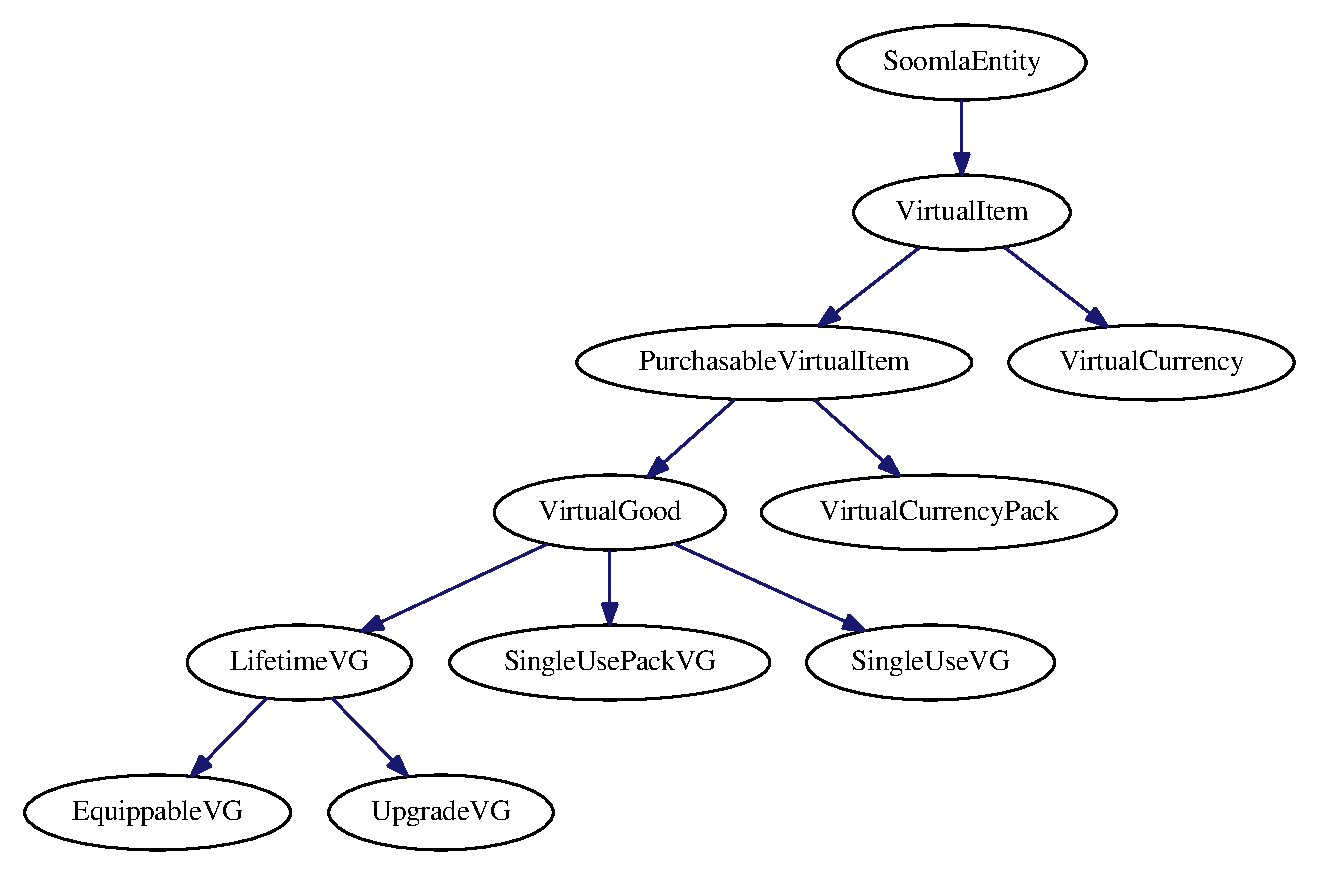
\includegraphics[width=\textwidth,draft=false]{images/soomla1.eps}
%\includegraphics[width=\textwidth,draft=false]{images/soomla4.eps}
%\caption{\label{gra1} \footnotesize\textbf{Distribution of the number of nodes in hierarchies} - The number of nodes composing the graphs has a power law distribution. The exponent $\sim x^{-2}$ is universal despite differences between the three languages.}
%\vspace{1cm}
%\includegraphics[width=\textwidth,draft=false]{images/soomla2.eps}
\caption{\label{gra1} \footnotesize\textbf{Example of hierarchical inheritance structure} - This is one of the graphs contained in the project Soomla Cocos2dx.}
\end{figure}
\newpage

\subsection{Data conversion}
Hierarchies reconstruction have been done by a series of scripts (see \ref{app} for examples) and with the aid of Doxygen \cite{doxy}, a program for code documentation.

Doxygen is not written with the goal of reconstructing inheritance hierarchies, but it gives you the chance of obtaining, for each class, a graph which reconstructs the hierarchy of the class \textit{upward} (any sister-classes are not included in graph). Cutting and pasting all the pieces of graphs, one can rebuild the whole hierarchy. This step has been done with the aid of gvpr, an \textit{awk} \cite{awk} inspired programming language useful for graphs manipulation.

Once obtained the hierarchies in the standard graphs format (.dot), finally the data have been converted in adjacency lists.

To analyze adjacency lists I have written a C++ library (see \ref{libra}) that allows the characterization of graphs (to calculate depth, to find roots and leaves, to assign levels to each node, to find eventually nodes not connected, \dots) and allows to obtain all principal statistical quantities, distributions and scatterplots.

To complete the analysis, I have written some C and bash scripts and lots of Gnuplot scripts to graphical the representation of the results.

\subsection{Templates and bias}
Analyzing converted data I came across some problems about their structure and composition.

For example, Doxygen consider as inheritance even the relation among a template class and all instances of its template variable. Since I don't consider such relation as inheritance, I wrote a script to exclude fake links among classes.

The second important problem was about data redundancy. Due to the sharing nature of open source code, it often happens that some big libraries are contained in slightly different versions in many packages. I can't exclude all redundancy from data, but I made some general controls to exclude packages that caused the most obvious bias. Instead, I considered good packages those whose libraries are not comparable to the naked eye, since they contain information useful for my analysis.

%******************************************************************************************************************************
\begin{figure}[p]%
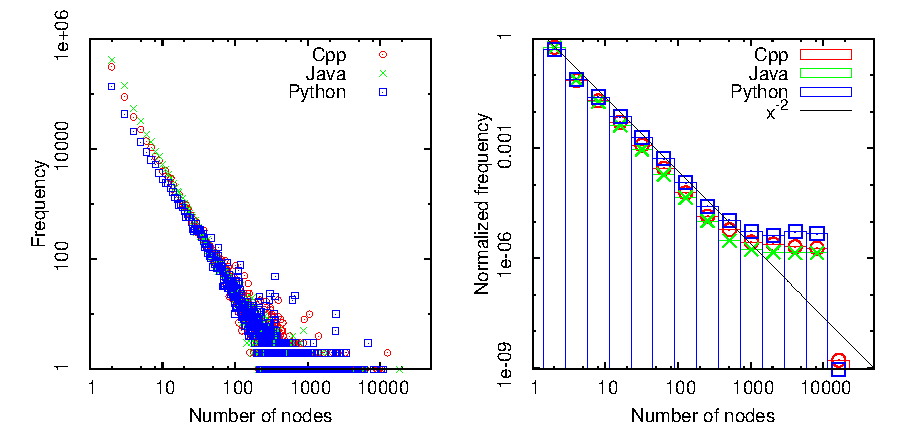
\includegraphics[width=\textwidth,draft=false]{grafici/fDNnodes.eps}
\caption{\label{Fnodes} \footnotesize\textbf{Distribution of the number of nodes in hierarchies} - The number of nodes composing the graphs has a power law distribution. The exponent $\sim x^{-2}$ is universal despite differences between the three languages.}
\vspace{1cm}
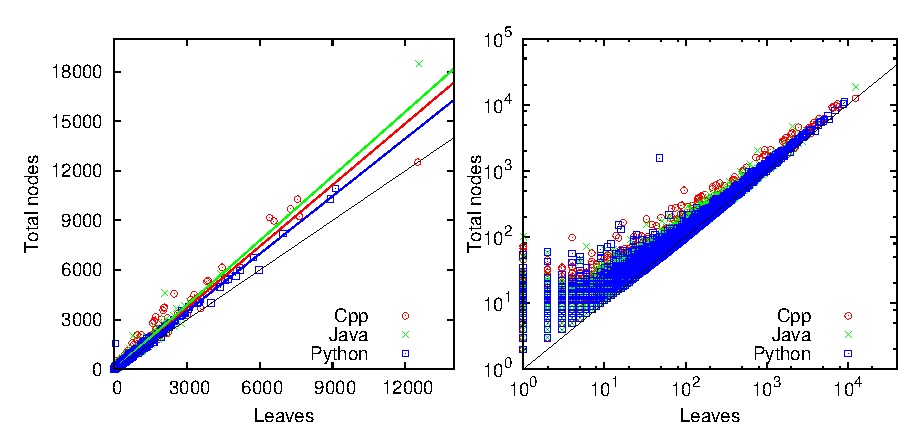
\includegraphics[width=\textwidth,draft=false]{grafici/leavesnodes.eps}
\caption{\label{Fleanodes} \footnotesize\textbf{Leaves and total nodes} - If a point (representing a graph) is near the black line, it means that almost all nodes of the graph are leaves, and so that only few nodes contain the shared code, while lots of classes inherit it.}
\end{figure}

\section{Graphs sizes}
The first important approach to noisy data is the sizes distribution. Graphs sizes and complexity is in some way coupled with the complexity of problems for which the whole set of programs is made for. In this thesis, I am not investigating the \textit{problems space}, that is true head of such distribution, but the whole following analysis will feel the consequences of sizes distribution.

The size of a directed acyclic graph can be defined in different ways. For our purposes, it is important to consider two main quantities: the number of nodes (and so of classes) which is the effective representation of hierarchy purpose, and the depth of graphs, which is the amount representing the hierarchies optimization.

\subsection{Solutions sizes}
Consider each hierarchy as the solution for a computer science problem, or task. How many classes are necessary to solve problems?

First of all, we analyze the total number of nodes of each graph (i.e. the number of classes of each hierarchy), the most important quantity to define the size of structures.

Plotting this quantity for each graph for each package, as showed in figure \ref{Fnodes}, we find a power law distribution with a small exponent ($\sim x^{-2}$).

Despite the differences among C++, Java and Python, this behavior is universal: hierarchies sizes are distributed in the same way, regardless the language in which they are built. This is the first interesting result that arise from the analysis: in principle, programming languages can be used to perform different tasks and they are designed in different ways and for different purposes. This seems not to influence the structure of inheritance hierarchies, at least in sizes distribution.

\begin{figure}[p]%
\includegraphics[width=\textwidth,draft=false]{grafici/fDdepth.eps}
\caption{\label{Fdepth} \footnotesize\textbf{Distribution of depth of each hierarchy} - While C++ and Python have the same power law distribution ($\sim x^{-5}$), Java structures are systematically less deeper than other languages.}
\vspace{1cm}
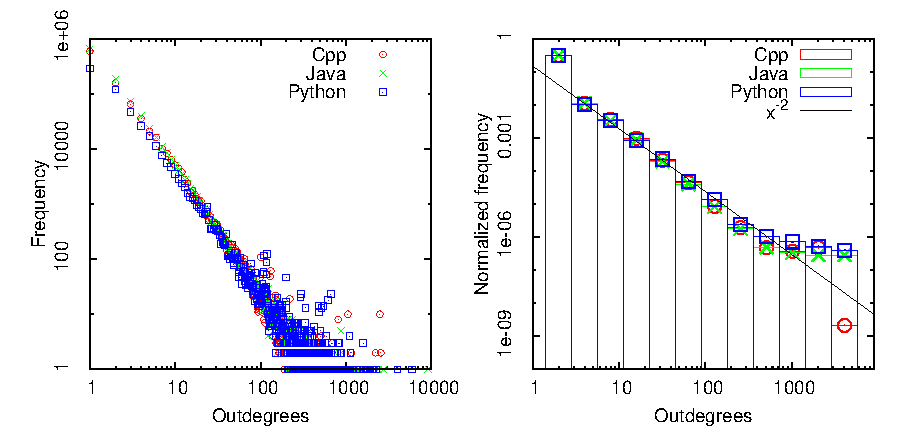
\includegraphics[width=\textwidth,draft=false]{grafici/fDoutdeg.eps}
\caption{\label{Foutdeg} \footnotesize\textbf{Distribution of outdegrees of all nodes of all graphs} - The outdegree quantifies the number of classes that inherits code from the same class. Its power law behavior can be caused by the power law distribution of the number of nodes of each graph, showed in figure \ref{Fnodes}. }
\end{figure}

\subsection{Sharing classes}
Not all classes of a hierarchy are directly used in programs: for example, abstract classes cannot be instantiated, and in general some classes can be built for sharing code purposes, abstracting concepts in \textit{super classes}.

While, in first approximation, we cannot know if an internal node is used or not, we can be sure that the leaves of each hierarchy are instantiable and that such classes are made to solve the task.

How many are the leaves compared to the total number of classes? How many classes share their code?

The answer is shown in figure \ref{Fleanodes}: the vast majority of classes in each hierarchy are leaves, i.e. classes that can be used in programs.

This result give us an important clue to argue that inheritance graphs take place only for high abstractability. If almost all nodes are leaves, as happens in the data, only few nodes are responsible of the collection of all the code that can be shared, while many nodes inherit it. The shared code must be useful for lots of classes, and lots of classes must hold something in common.

This behavior makes us also to think about a general small depth of graphs, and in next section we will check it.

\subsection{Depth of hierarchies}
Hierarchies depth is a surprisingly small quantity: also the largest structures have at most eleven or twelve levels, while the vast majority of graphs have a depth equal to two or three. This result is the second clue that supports the idea for which abstractability is high in all real hierarchies.

Another important result given by figure \ref{Fdepth} is that Java language does not behave as C++ and Python: depths distribution of Java hierarchies is consistently below the other two distributions. The reasons of this discrepancy can be found directly in Java inheritance implementation rules. In Java, multiple inheritance is allowed only by a special kind of relation given by the keywords \textit{interface} and \textit{implements}. \textit{Interface} is the kind of class that can be inherited without limitations about the multiple inheritance, but \textit{implements} is the keyword that the class which inherits the interface must have: an interface cannot contains \textit{implementation}, but only declarations of methods and functions. The reasons for which a class inherits from interfaces is code reuse as well, but not in the sense expressed by models in sections \ref{Ceffort} and \ref{CTree}.

This and other features have been inserted in Java language in order to obtain a simpler and more safe programming. We can expect other differences in data between Java and the other two languages. We can say that Java inheritance rules give rise to less deeper hierarchies respect to other languages (especially C++ from which Java is developed), and in this sense they have a simplified effect as hoped by Java designers.

%******************************************************************************************************************************
\begin{figure}[p]%
\includegraphics[width=\textwidth,draft=false]{grafici/fDindeg.eps}
\caption{\label{Findeg} \footnotesize\textbf{Distribution of indegrees of all nodes of all graphs} - Indegrees are systematically less than outdegrees and distributions have a strong cutoff, especially for Java hierarchies.}
\vspace{1cm}
\includegraphics[width=\textwidth,draft=false]{grafici/depVSNnodes.err.eps}
\caption{\label{FdVSnerr} \footnotesize\textbf{Depth VS Nnodes } - Depth of graphs seems a logarithmic function of the number of object for C++ and Python, while the depth is almost constant in Java hierarchies. The fit for C++ and Python give $y \sim 0.5\log(x)+1.5$}
\end{figure}

\section{Code shareability}
The outdegree quantifies the number of classes that inherit code from the same class. The power law distribution of graphs sizes affects outdegrees distribution (over all nodes of all graphs), which appears as a power law with the same exponent ($\sim x^{-2}$). This is not a surprising result, since regardless the outdegrees distribution of each graph, its sum over all graphs (which sizes are power law distributed) will have a power law shape as well. See figure \ref{Foutdeg}.

For this reason, it's important to look at outdegrees distribution of each graph. Is the outdegrees distribution a real power law or it is an effect caused by the sizes?

As showed in figure \ref{Finoutd}, the power law appears as distribution of outdegrees also in single graphs, at least for biggest hierarchies. Outdegrees distribution is therefore the results of the sum of many power laws.

%fare grafico con l'esponente della powerlaw dell'outdeg VS numero di nodi? sono tutte powerlaw davvero'
%******************************************************************************************************************************
\section{Tree approximation}
Models presented in sections \ref{CTree} and \ref{Ceffort} schematize hierarchies through trees, while inheritance structures can be in principle directed acyclic graphs. The main difference between this two kind of graphs is in the number of indegrees of each node: if a graph is a tree, all nodes can have at most one indegree, while indegrees have no restrictions for a directed acyclic graph.

In programming languages, multiple inheritance is often not recommended, except in cases where actually required. In data we can observe multiple inheritance, but it is systematically less than single inheritance, as expected. When indegrees distribution is compared to outdegrees distribution in a hierarchy, as in figure \ref{Finoutd}, one can observe how outdegree is the first main quantity to keep into account in an object-oriented hierarchy model.

The outdegrees distribution shows power law behavior with a small exponent ($\sim x^{-2}$ or even less), while indegrees distribution shows a power law behavior with a large exponent ($\sim x^{-3}$ and often more), large enough to allow a first approach considering the indegree constant and equal to its mean, that is about $1$. In this sense, tree approximation is an excellent first approach to this system.

Distribution of indegrees of all nodes of all graphs shows a power law behavior, with exponent $\sim x^{-3}$ (see figure \ref{Findeg}). The three programming languages have quite different behaviors. In Python only the $0.1\%$ of nodes has outdegree greater than one and no one class has more than $300$ indegrees. In Java, indegrees are often more respect to other languages, as expected from an \textit{interfaces programming}, but all class has less than $100$ indegrees. In C++ indegrees can reach $1000$ classes.

\begin{figure}[p]%
\includegraphics[width=\textwidth,draft=false]{grafici/cppinout.eps}
\includegraphics[width=\textwidth,draft=false]{grafici/javainout.eps}
\includegraphics[width=\textwidth,draft=false]{grafici/pyinout.eps}
\caption{\label{Finoutd} \footnotesize\textbf{Comparison between indegrees and outdegrees} - The different exponent for indegree and outdegree in each graph shows how tree approximation is an excellent first approach to this system.}
\end{figure}

%******************************************************************************************************************************
\section{Lateral growth}
Graphs are complex structures and their topology has lots of features. A way to give a summary look into its shape is asking in which way the depth is coupled to the number of objects in hierarchies, in order to have an idea about the ratio of the \textit{vertical} dimension (i.e. the depth) and the \textit{horizontal} dimension (i.e. the number of objects in levels).

\subsection{Horizontal and vertical dimensions}
Plotting the depth versus the number of objects for each graph allow to reconstruct a distribution of occurrence for each programming language, which means and standard deviations are showed in figure \ref{FdVSnerr}.

Python and C++ behave in the same way: the depth is in good approximation a logarithmic function of the number of objects (at least for most of sizes). For Java hierarchies, instead, the depth is almost a constant function of the number of classes that grows only for big graphs sizes. Both results are descriptive of a \textit{later growth} of graphs instead of a vertical one.

Consider two hierarchies with a very different number of objects. Despite the gap between the two effective sizes of the structures, we may expect two graphs with similar depths, at most one increased or decreased by one respect the other, especially for Java structures.

The logarithmic behavior of the depth as a function of the number of objects is well captured by the Sharing Tree model and the Effort model. Both mean field hierarchies and simulated trees well describe this feature.

\subsection{Shallow is better}
A really interesting result is the change in behavior of the depth as a function of the number of objects, as highlight in figure \ref{FdVSnheat} through a heat map for each programming language. 

In object-oriented programming languages there are general advices that suggest to keep hierarchies as shallow as possible, in order to avoid the anti-pattern known as \textit{Yo-yo problem} \cite{yoyo}. If inheritance graph is too much long and complicated, then a programmer that has to read and understand the hierarchy, has to keep flipping between different parts of the code.

For these reasons, the huge amount of shallow hierarchies was foreseeable. But what happens when hierarchy size get over $1000$ classes?

The artificial attempt to keep hierarchies as shallow as possible seems to fail, and all hierarchies show a depth greater than that expected.

Can the guess for which \textit{shallow is better} be wrong? If shallow hierarchies are produced by a false assumption, can the optimization be achieved through deep hierarchies?

\begin{figure}[p]%
\includegraphics[width=\textwidth,draft=false]{grafici/Heatmap.cpp.eps}
\includegraphics[width=\textwidth,draft=false]{grafici/Heatmap.java.eps}
\includegraphics[width=\textwidth,draft=false]{grafici/Heatmap.py.eps}
\caption{\label{FdVSnheat} \footnotesize\textbf{Depth VS nodes in C++, Java and Python hierarchy} - Colors (used in log scale) are representative of how many graphs have the $x$ number of nodes and depth equal to $y$. Colors represent the whole distribution, while lines trace the mean. Comparison of this three trends is given in figure \ref{FdVSnerr}. }
\end{figure}

%******************************************************************************************************************************
\section{Vertical balancing}
Inspired by models, we can investigate more accurately the topology of hierarchies studying the behavior of the outdegree mean of nodes as a function of the levels. Is it constant across graphs? If not, where are situated objects with the most shared code?

\subsection{Code shareability per level}
Once established that graphs are wider than high, we can probe the \textit{vertical balancing}. An interesting quantity that we can study as a function of a vertical variable (i.e. of levels) is the outdegree mean of nodes.

When the outdegree is high, the code contained in classes is shared with lots of other classes: high outdegree means high shareability.

Some examples of this function are given in figures \ref{Foutdegcpp} and \ref{Foutdegjp}. We can observe that the outdegree mean is a quantity that tends to grow with levels, with pronounced peaks close to the root. 

Why this behavior? Why the outdegree mean grows with level?

\begin{figure}[ht]%
\includegraphics[width=\textwidth,draft=false]{grafici/Coutdeg.cpp2.eps}
\caption{\label{Foutdegcpp} \footnotesize\textbf{Outdegree mean for Cpp hierarchies} - Examples of structure with more than 1000 nodes and depth equal to 6, 7 and 8 (in order).}
\end{figure}

\begin{figure}[hp]%
\includegraphics[width=\textwidth,draft=false]{grafici/Coutdeg.java.eps}
\includegraphics[width=\textwidth,draft=false]{grafici/Coutdeg.py.eps}
\caption{\label{Foutdegjp} \footnotesize\textbf{Outdegree mean for Java and Python hierarchies} - In the upper side figures, examples of Java structure with more than 500 nodes and depth equal to 4, 5 and 6 (in order). The other figures represent examples of python structure with more than 500 nodes and depth equal to 6, 7 and 8 (in order).}
\end{figure}

\subsection{Shallow regime}
Thanks to the mean field model (Effort model), we can give an interpretation to the growth of outdegree with levels.

We have showed in chapter \ref{Ceffort} how the outdegree mean behavior, as function of levels, is very sensible to \textit{depth constrain} and that it can have a strong growth close to the root in the case of insufficient depth. This is exactly the situation in which we find inheritance hierarchies in data.

This is yet another clue that leads us to argue that \textit{shallow hierarchies} are not the best solution. Code reuse appears not optimized by a decrease of the depth in Effort model, and data appears as trapped in an artificial \textit{shallow regime}.

A most efficient documentation system could avoid the \textit{yo-yo problem} as well as decreasing the depth of hierarchies, without sacrificing the optimal depth.

%******************************************************************************************************************************
\section{Optimal or random?}
The models proposed in this thesis are based on the assumption that inheritance graphs are made with optimizing spirit. This is a perfectly reasonable assumption since there are no reasons to hypothesize that inheritance arise from chaos.

Anyway, it is interesting to compare Sharing Tree graphs with graphs obtained through models completely random and made without optimization mechanisms.

\subsection{Random Branching Tree model}
A Random Branching Tree can be built starting from an initial node, the root, and choosing a distribution with a well-defined mean.

As a first step, we extract a random variable from the distribution: the extraction represents the root outdegree and so the number of nodes that are connected to the root. Once added new nodes, the process is iterated for each new node until a certain condition is reached.

The outdegree mean in function of levels is obviously a constant value, equal to the mean of the chosen distribution for the outdegree. Simulations are shown in figure \ref{Foutrpm}.

Which random mechanism can be introduced to obtain a non constant function? 

\begin{figure}[p]%
\includegraphics[width=\textwidth,draft=false]{grafici/Coutdeg.yul.eps}
\includegraphics[width=\textwidth,draft=false]{grafici/Coutdeg.rus.eps}
\caption{\label{Foutrpm} \footnotesize\textbf{Random branching tree and Pang-Maslov models simulation} - The outdegree mean in function of levels does not reproduce the behavior observed in data.}
\end{figure}

\subsection{Pang-Maslov model}
The Pang-Maslov model \cite{pangmaslov} can be used to construct a tree. Consider an initial node an a process for which, at each step, a new node arrives and sticks to one of the existing nodes. The process can be iterated until a certain condition is reached.

This model prevents the constancy of outdegree mean, since the older nodes have had more chance of being chosen by another node, and so they must have an outdegree greater than young nodes. Growth, however, is constant and it does not represent well the behavior of outdegree mean in data.

\subsection{Sharing Tree comparison}
Through the Sharing Tree model, we can can produce Monte Carlo trees to explicitly compare optimization ideas with data. Some examples are given in figure \ref{STsim}.

The outdegree mean has not a trivial behavior due to its strong growth close to the root, that is also the main feature observable in data.

Therefore, there is a very good agreement between data and optimization models.

\begin{figure}[htp]%
\includegraphics[width=\textwidth,draft=false]{grafici/STsim.eps}
\caption{\label{STsim} \footnotesize\textbf{Sharing Tree Monte Carlo simulations} - The Sharing Tree model well capture the behave of the outdegree mean as function of levels. In simulations, parameters are $\Enne=1000$, $\kappa=100$ and $\Esse=2000$.}
\end{figure}

